\documentclass[a4paper, 12pt]{scrartcl}
\usepackage{listings}
\usepackage{color}
\usepackage{graphicx}
\usepackage{hyperref}
\lstdefinelanguage{XML}
{
  basicstyle=\ttfamily\footnotesize,
  morestring=[b]",
  moredelim=[s][\bfseries\color{blue}]{<}{\ },
  moredelim=[s][\bfseries\color{blue}]{</}{>},
  moredelim=[l][\bfseries\color{blue}]{/>},
  moredelim=[l][\bfseries\color{blue}]{>},
  morecomment=[s]{<?}{?>},
  morecomment=[s]{<!--}{-->},
  commentstyle=\color{black},
  stringstyle=\color{blue},
  identifierstyle=\color{red}
}

\setkomafont{sectioning}{\rmfamily}

\title{XML Technologies: Exercise 5}
\date{}
\subtitle{XSL-FO, XML Parsing}
 
\begin{document}
\maketitle\vspace{-12ex}

\noindent This is a mandatory exercise and the result will be part of your final mark. The solution must be uploaded to OLAT by \textbf{April 29\textsuperscript{th} at 15:59}. Late submissions will not be accepted.\\


\noindent Submit the following files in a zipped archive:
\begin{itemize}
\item xwing.xsl, xwing.fo, xwing.pdf
\item answers.txt
\end{itemize}

\noindent Make sure the archive is named [lastname]\_[firstname]\_5.zip (for example \textit{mueller\_mathias\_5.zip}). Some parts of your submission may be automatically evaluated, so make sure to name your files \textit{precisely} as prescribed, otherwise you might not get any points.

\section{An XML-Wing Fighter (3 Points)}

XSL-FO is a \textit{presentational} markup language. It is written in XML, which has the following advantages:

\begin{itemize}
\item XSL-FO documents can easily be generated with XSLT (in fact, that's the most common way to create XSL-FO),
\item can easily be manipulated and queried by any XML technology,
\item and, most importantly, other markup languages can easily be woven into XSL-FO -- in their own namespaces, of course.
\end{itemize}

\noindent In this exercise, we are going to exploit this last fact, namely that XSL-FO easily mixes with other kinds of XML. We will transform content from two different XML documents into XSL-FO and finally render it as PDF.

\subsection{Input Documents}

The first input documents is \texttt{xwing.svg}, which is an SVG file. The purpose of SVG is to provide a means to create graphics that are \textit{scalable}, i.e. that do not have a fixed resolution, very unlike most graphics formats. Therefore, a rendering agent like a web browser can display an SVG graphic in any size.\\

\noindent Check the attached \texttt{sample.svg} to get an idea of what a simple SVG file looks like. Pay special notice to attributes such as \texttt{fill="\#7DD8B5"}, which indicate how elements are coloured. \\

\noindent The second input document \texttt{xwing-wiki.xml} is a very simple snippet from Wikipedia. \\

\subsection{Transforming Input Documents to XSL-FO and Rendering as PDF}

\noindent Generally, XSLT is used to generate an FO file, which is then rendered into PDF. \\

\noindent \textbf{Using the \texttt{scaffold.xsl} provided, fill in the blanks to create a FO document, which:}

\begin{itemize}
\item \textbf{First shows the SVG image}
\item \textbf{Then shows the text for every \texttt{<p>}-element in the \texttt{xwing-wiki.xml}}
\end{itemize}


\noindent \textbf{Then render the resulting XSL-FO document as PDF.} The resulting PDF should look very similar to the picture below. \\

\begin{center}
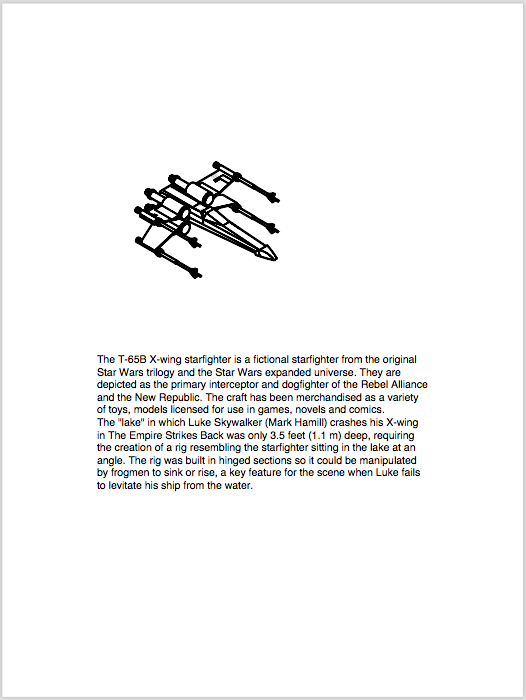
\includegraphics[width=8cm]{attachments/picture-below.png}
\end{center}

\noindent \textbf{Save your XSLT stylesheet as \texttt{xwing.xsl}, your XSL-FO file as \texttt{xwing.fo} and the rendered PDF as \texttt{xwing.pdf}.}


\section{Parsing XML (2 Points)}

XML documents are merely text files stored in the file system. Before an application can access the contents of an XML document, the document must be \textit{parsed}. Roughly speaking, there are two different ways to parse XML -- DOM and SAX -- and they have fundamental differences. \\

\noindent \textbf{Answer the following questions:
\begin{itemize}
\item DOM means ``document object model''. What does that mean? Why is it sometimes called a \textit{tree}?
\item Which method uses a lot more RAM? Why?
\item Which of them is an event-driven and streaming method? Why?
\item Which of them is more suitable for use with XPath? Why? Substantiate your claim with an XPath expression, i.e. find an XPath expression which will not be possible to execute using both approaches.
\end{itemize}
}

\noindent \textbf{Answer in full sentences and save your answers as \texttt{answers.txt}.}



\end{document}